%\newcommand{\notatki}{1}
\documentclass{sa}
\usepackage{array} %dla poziomego wyrownania (m) w tabeli
\usepackage{soul}
\usepackage{bm}

\newcommand{\ang}[1]{(ang. \emph{#1})}
\renewcommand{\vec}[1]{\ensuremath\boldsymbol{#1}}
\newcommand{\grad}{\ensuremath\nabla}
\let\avg\overline

\usetikzlibrary{datavisualization}
\usetikzlibrary{datavisualization.formats.functions}

\usepackage{hyperref}
\graphicspath{{05_nn/}}
\subtitle{Sieci neuronowe}
\begin{document}
\begin{frame}
\titlepage
\end{frame}

\begin{frame}{Perceptron (Rossenblat, 1957)}
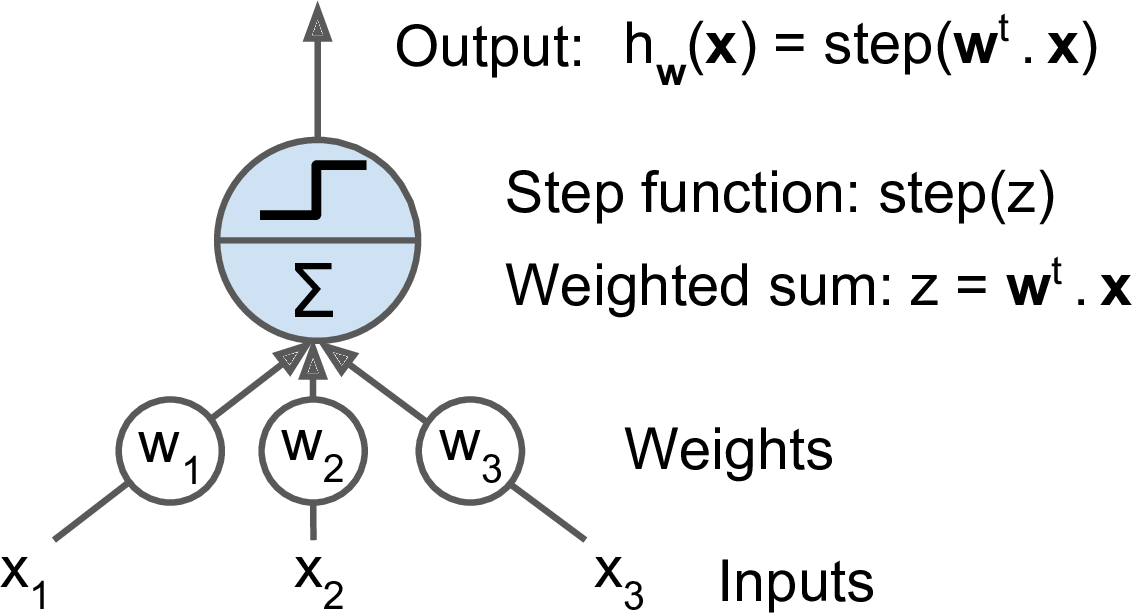
\includegraphics[width=\textwidth]{perceptron.png}
{\vfill\footnotesize A. Géron, \emph{Hands-On Machine Learning with Scikit-Learn and TensorFlow} 2017}
\end{frame}

\begin{frame}{Perceptron}
\begin{gather*}
step(z) = \begin{cases} 1 & z \geq 0 \\ 0 & \text{w przeciwnym przypadku} \end{cases} \\
\pause
\hat{y} = step(\vec{w}^T\vec{x}) \\
\pause
\hat{\vec{y}} = step(\vec{X}\vec{w})
\end{gather*}
\end{frame}

\begin{frame}{Perceptron z wieloma wyjściami}
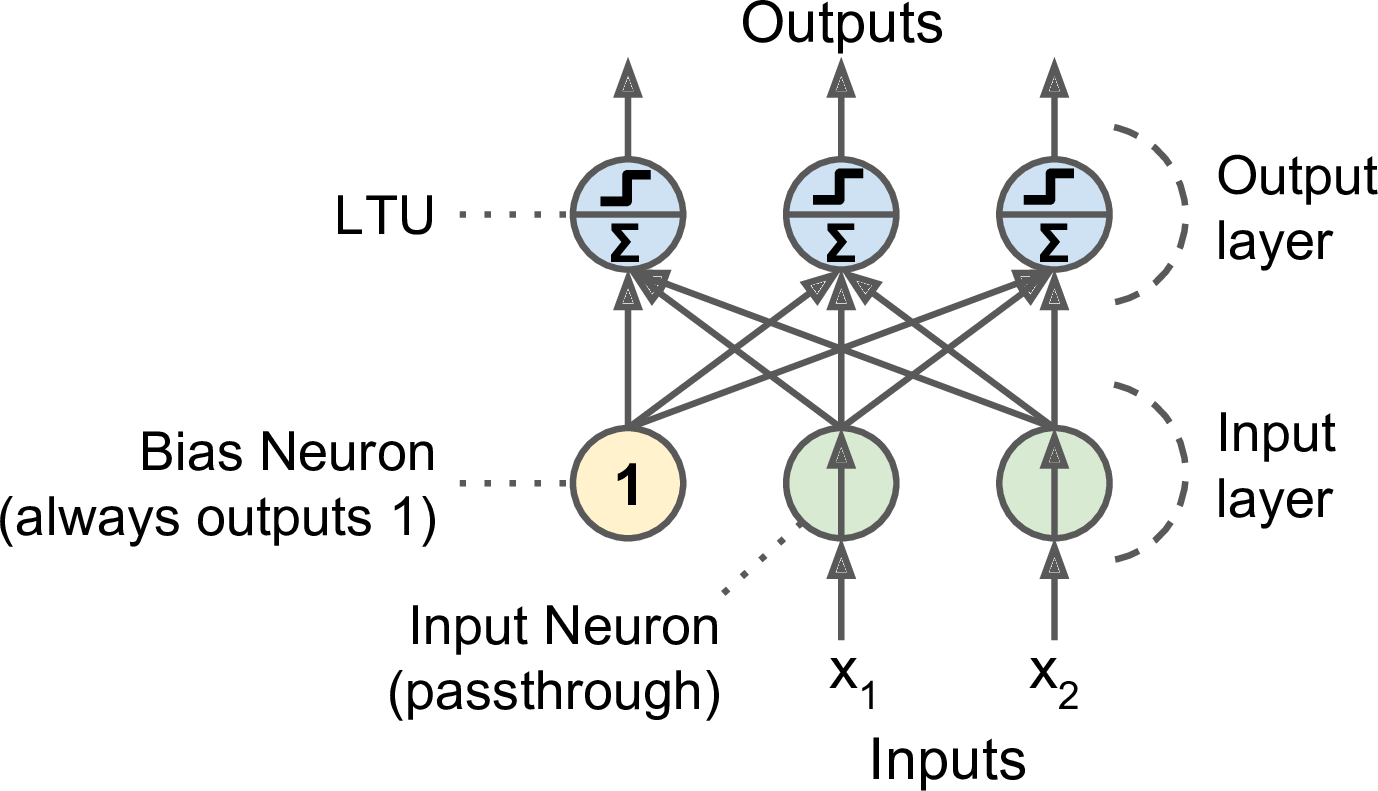
\includegraphics[width=\textwidth]{multioutput_perceptron.png}
{\vfill\footnotesize A. Géron, \emph{Hands-On Machine Learning with Scikit-Learn and TensorFlow} 2017}
\note<1>
{
LTU -- linear threshold unit
}
\end{frame}

\begin{frame}{Uczenie perceptronu}
\[ w_{i,j}^{(\varepsilon+1)} = w_{i,j}^{(\varepsilon)} + \eta(y_j-\hat{y_j})x_i \]
\begin{itemize}
\item $w_{i,j}$ waga połączenia między wejściem $i$, a wyjściem $j$
\item $\varepsilon$ krok
\item $\eta$ prędkość uczenia
\end{itemize}
\end{frame}

%TODO przykład na działanie perceptronu i regułę uczenia

\begin{frame}{AND}
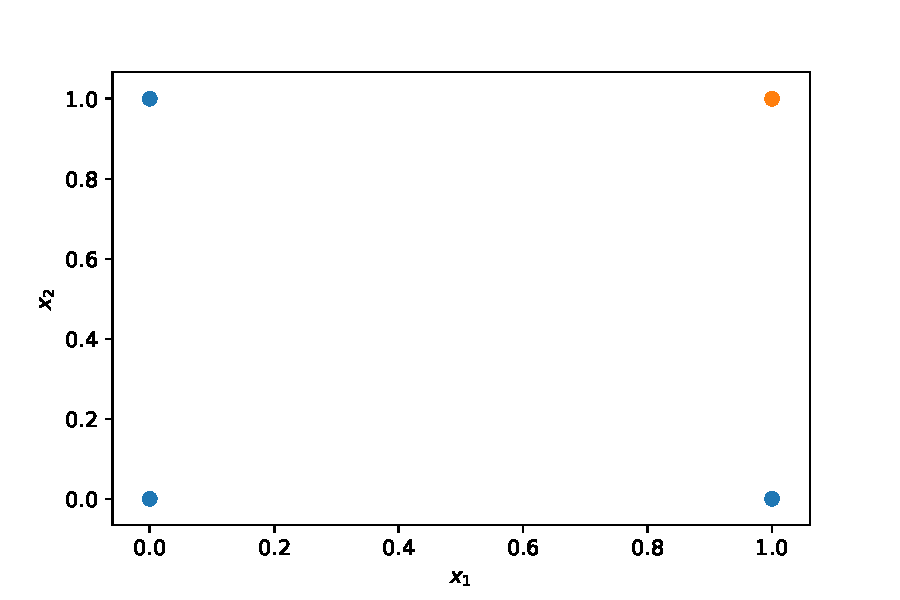
\includegraphics[width=.9\textwidth]{and.pdf}

\alert{Jakie wagi musi mieć perceptron, żeby rozwiązać taki problem?}
\note<1>
{
Na przykład $1x_1+1x_2-1.5$
\begin{tabular}{rrrr}
$x_1$ & $x_2$ & $z$ & $\hat{y}$ \\
0 & 0 & $-1.5$ & 0 \\
0 & 1 & $-0.5$ & 0 \\
1 & 0 & $-0.5$ & 0 \\
1 & 1 & $0.5$ & 1 \\
\end{tabular}
}
\end{frame}

\begin{frame}{XOR}
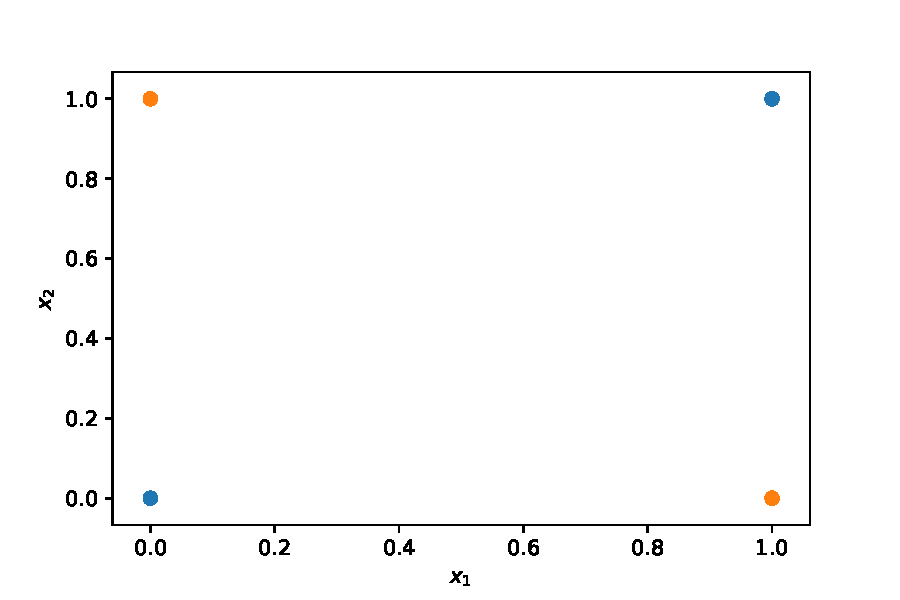
\includegraphics[width=.9\textwidth]{xor.pdf}

\alert{Jakie wagi musi mieć perceptron, żeby rozwiązać taki problem?}
\end{frame}

\begin{frame}{Perceptron wielowarstwowy (MLP -- multilayer perceptron)}
\begin{center}
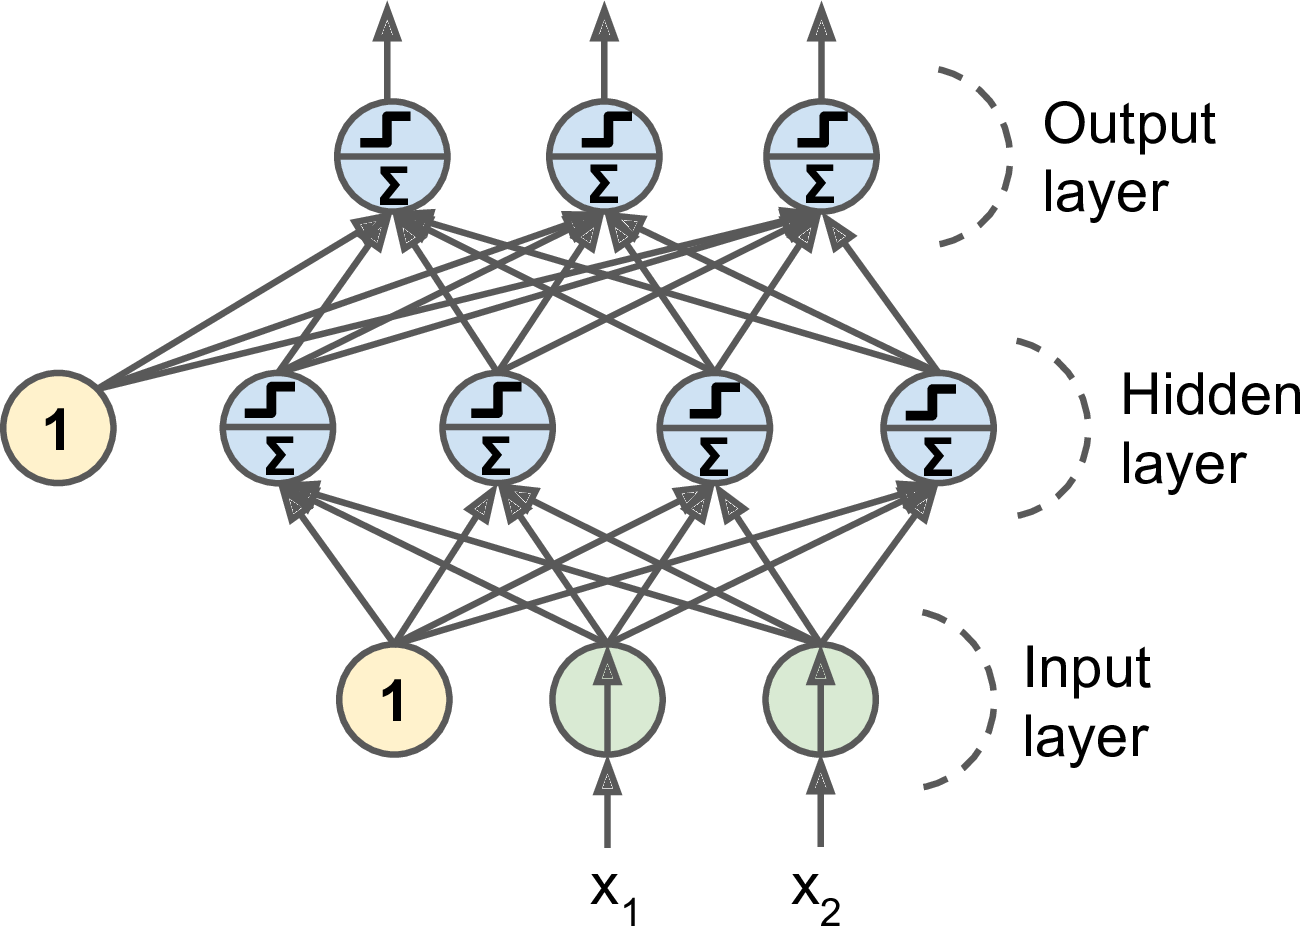
\includegraphics[width=.8\textwidth]{mlp.png}
\end{center}
{\vfill\footnotesize A. Géron, \emph{Hands-On Machine Learning with Scikit-Learn and TensorFlow} 2017}
\end{frame}

\begin{frame}{Jak to uczyć: backpropagation (Rumelhart et al.  1986)}
\begin{enumerate}
\item Oblicz wyjścia sieci
\item Oblicz błąd popełniony przez sieć
\item Korzystając z gradientu delikatnie zmodyfikuj wagi
\end{enumerate}
\pause
\alert{Wszystko proste, jasne i oczywiste?}
\end{frame}

\begin{frame}{Funkcja aktywacji}
\alert{Ile wynosi pochodna funkcji $step(z)$?}

\pause
Popularne funkcje aktywacji:
\begin{description}
\item[logistyczna] \[ \sigma(z) = \frac{1}{1+e^{-z}} \]
\pause
\item[tangens hiperboliczny] \[ \tanh(z) = 2\sigma(2z) - 1 \]
\pause
\item[ReLU (rectified linear unit)] \[ ReLU(z) = \max\{z, 0\} \]
\end{description}
\end{frame}

\begin{frame}{Funkcje aktywacji i ich pochodne}
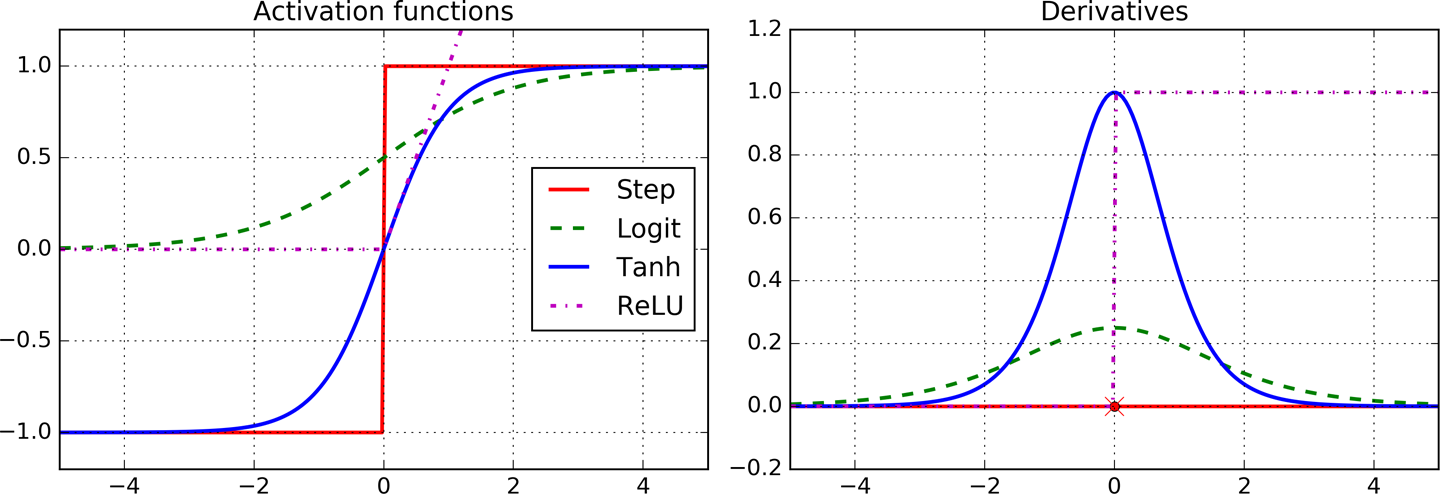
\includegraphics[width=\textwidth]{activation_functions.png}
{\vfill\footnotesize A. Géron, \emph{Hands-On Machine Learning with Scikit-Learn and TensorFlow} 2017}
\end{frame}


\begin{frame}{Graf obliczeń}
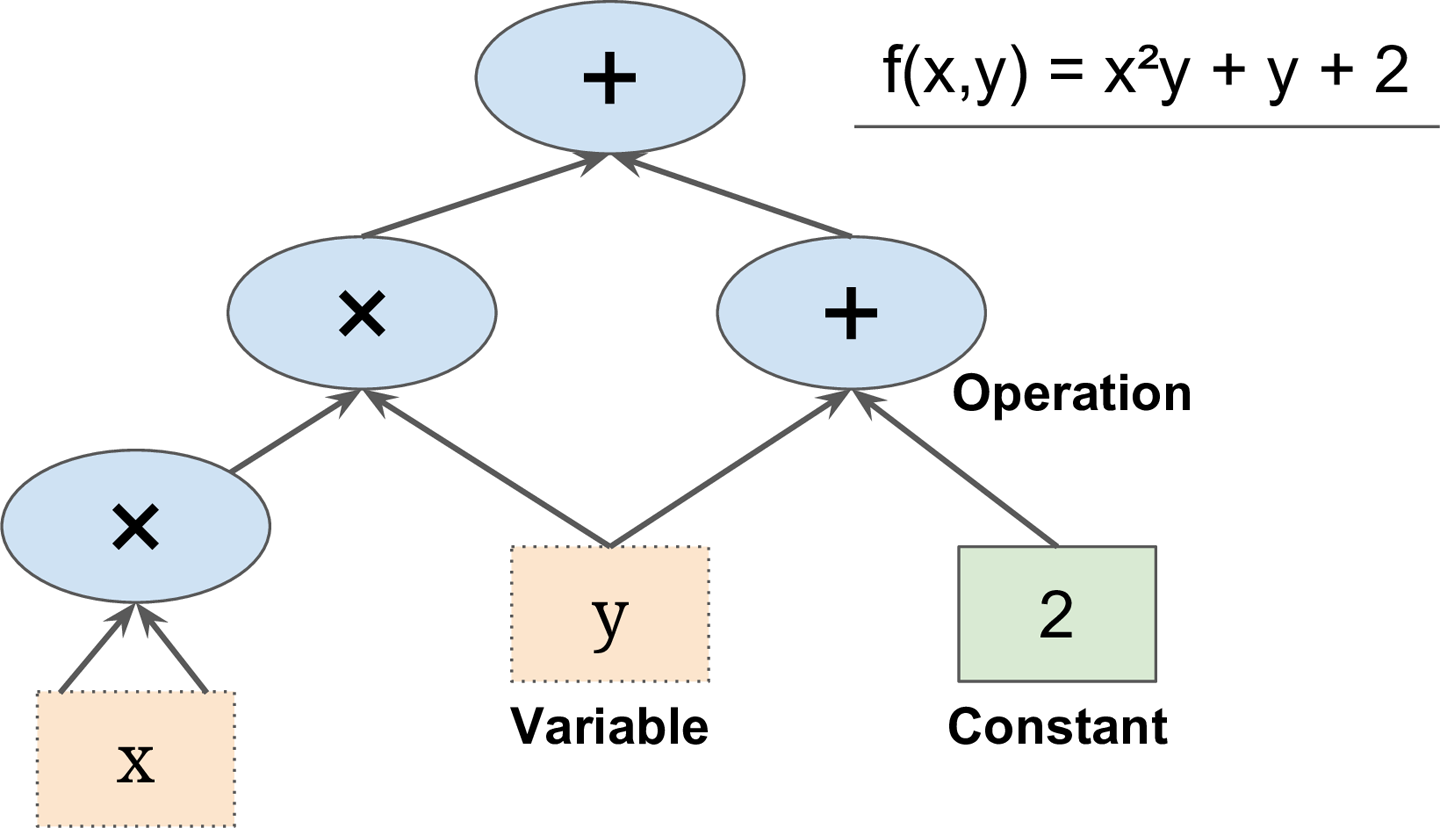
\includegraphics[width=\textwidth]{comp_graph.png}
{\vfill\footnotesize A. Géron, \emph{Hands-On Machine Learning with Scikit-Learn and TensorFlow} 2017}
\end{frame}

\begin{frame}{Reverse-mode autodiff}
\begin{center}
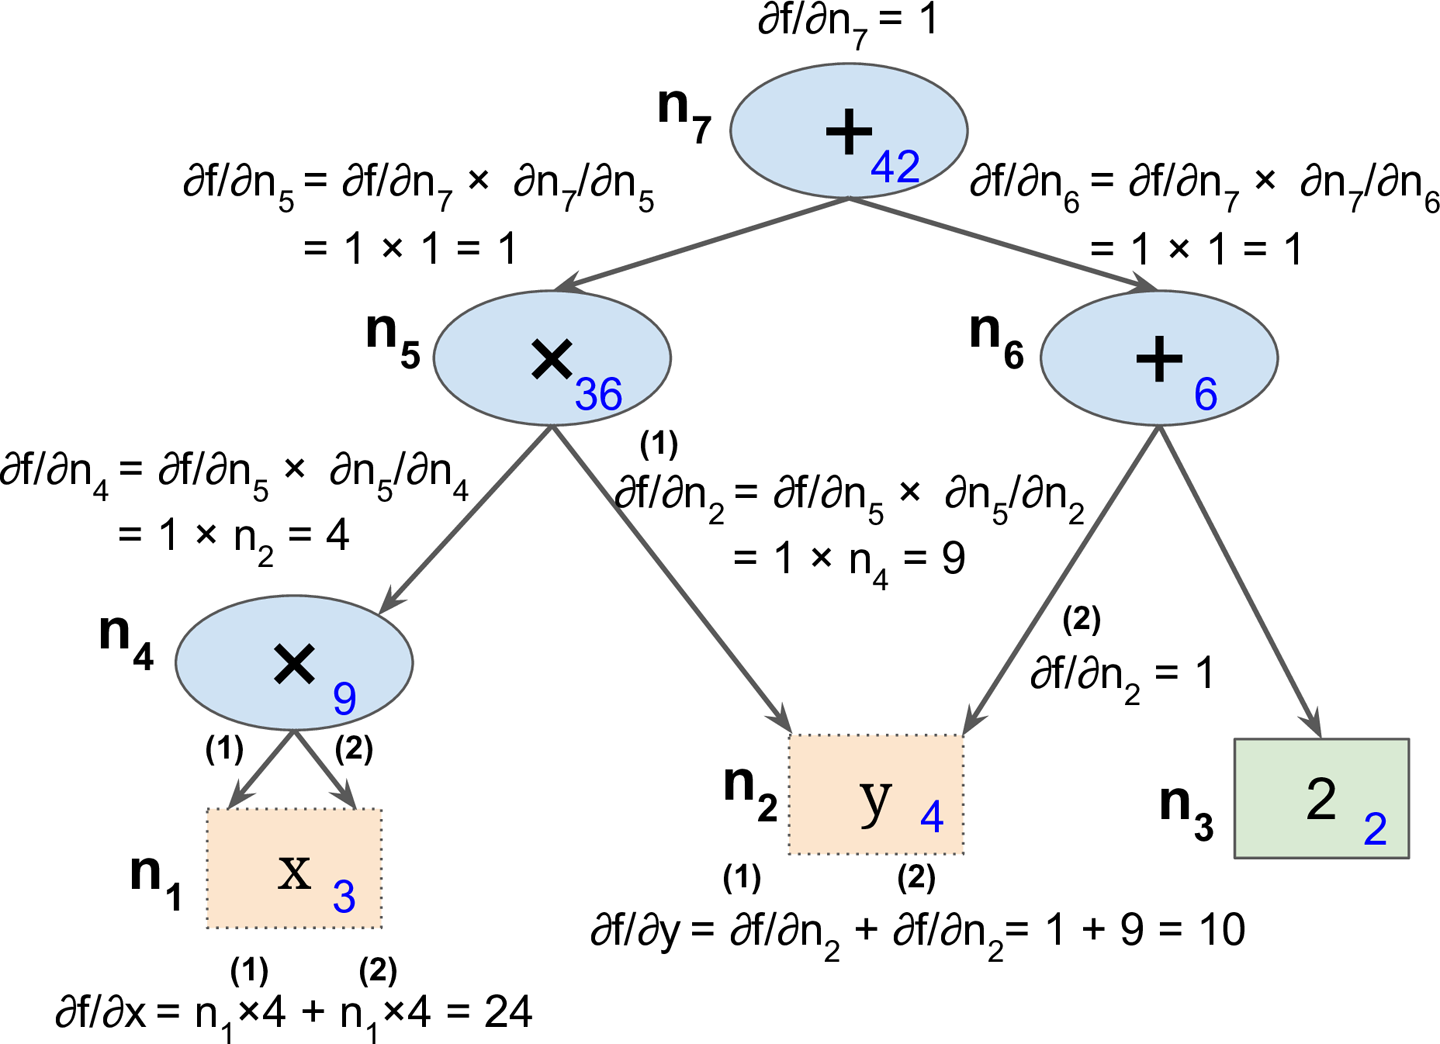
\includegraphics[width=.8\textwidth]{rev-mode_autodiff.png}
\end{center}
{\vfill\footnotesize A. Géron, \emph{Hands-On Machine Learning with Scikit-Learn and TensorFlow} 2017}
\end{frame}

\begin{frame}{Współczesna sieć neuronowa do klasyfikacji}
\centering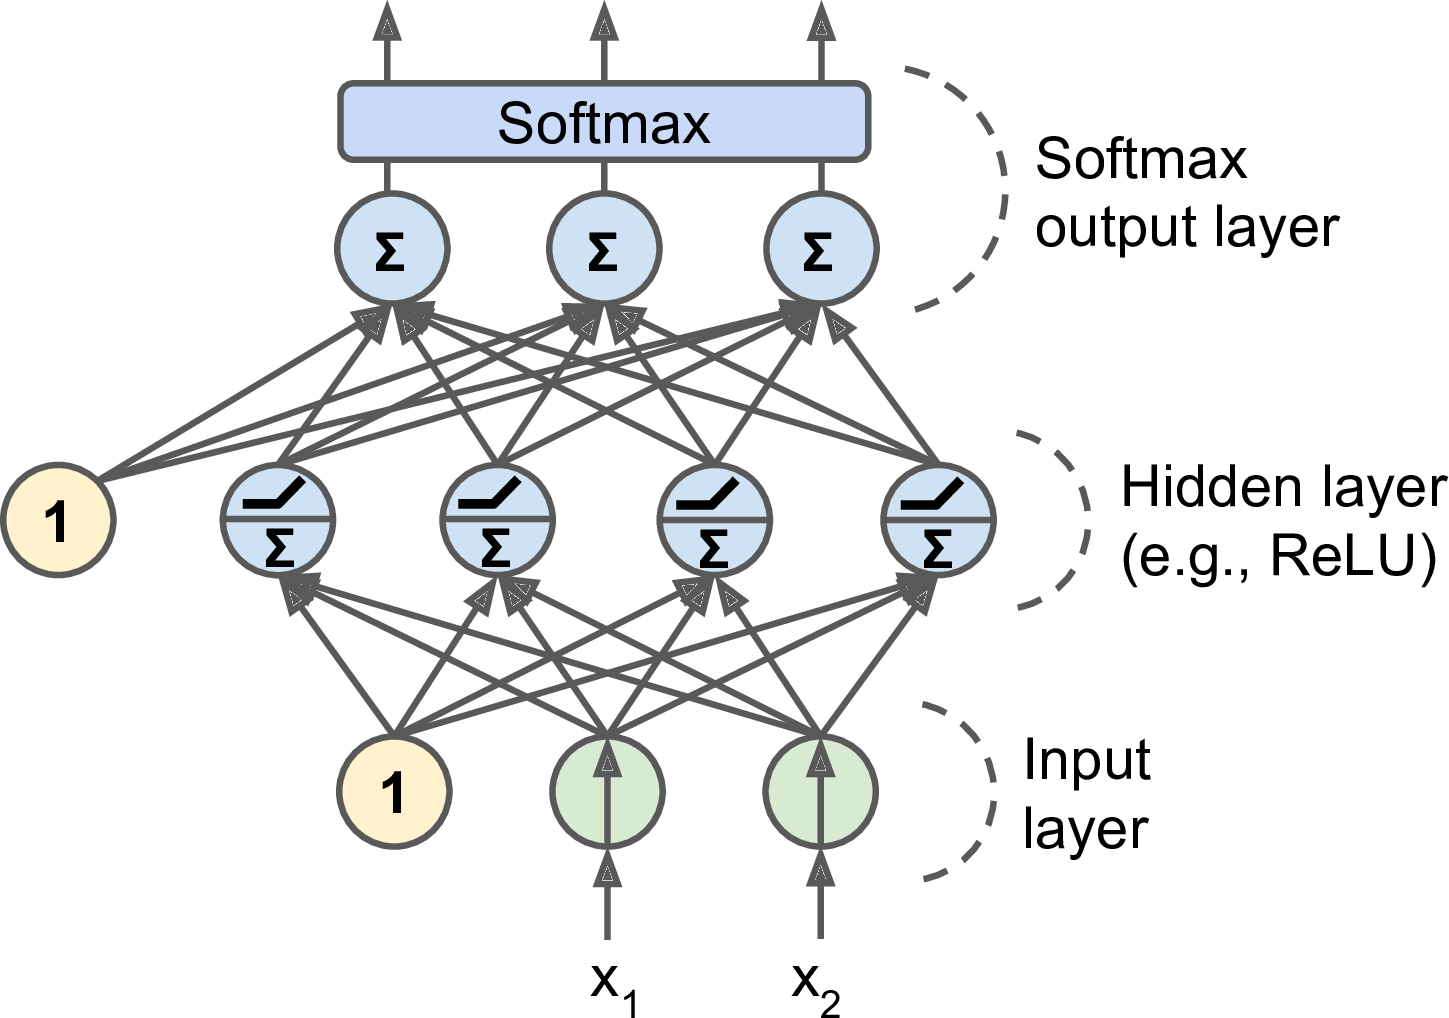
\includegraphics[width=.9\textwidth]{mlp_relu_softmax.png}
{\vfill\footnotesize A. Géron, \emph{Hands-On Machine Learning with Scikit-Learn and TensorFlow} 2017}
\end{frame}

\begin{frame}{Eksplodujący i znikający gradient}
\begin{center}
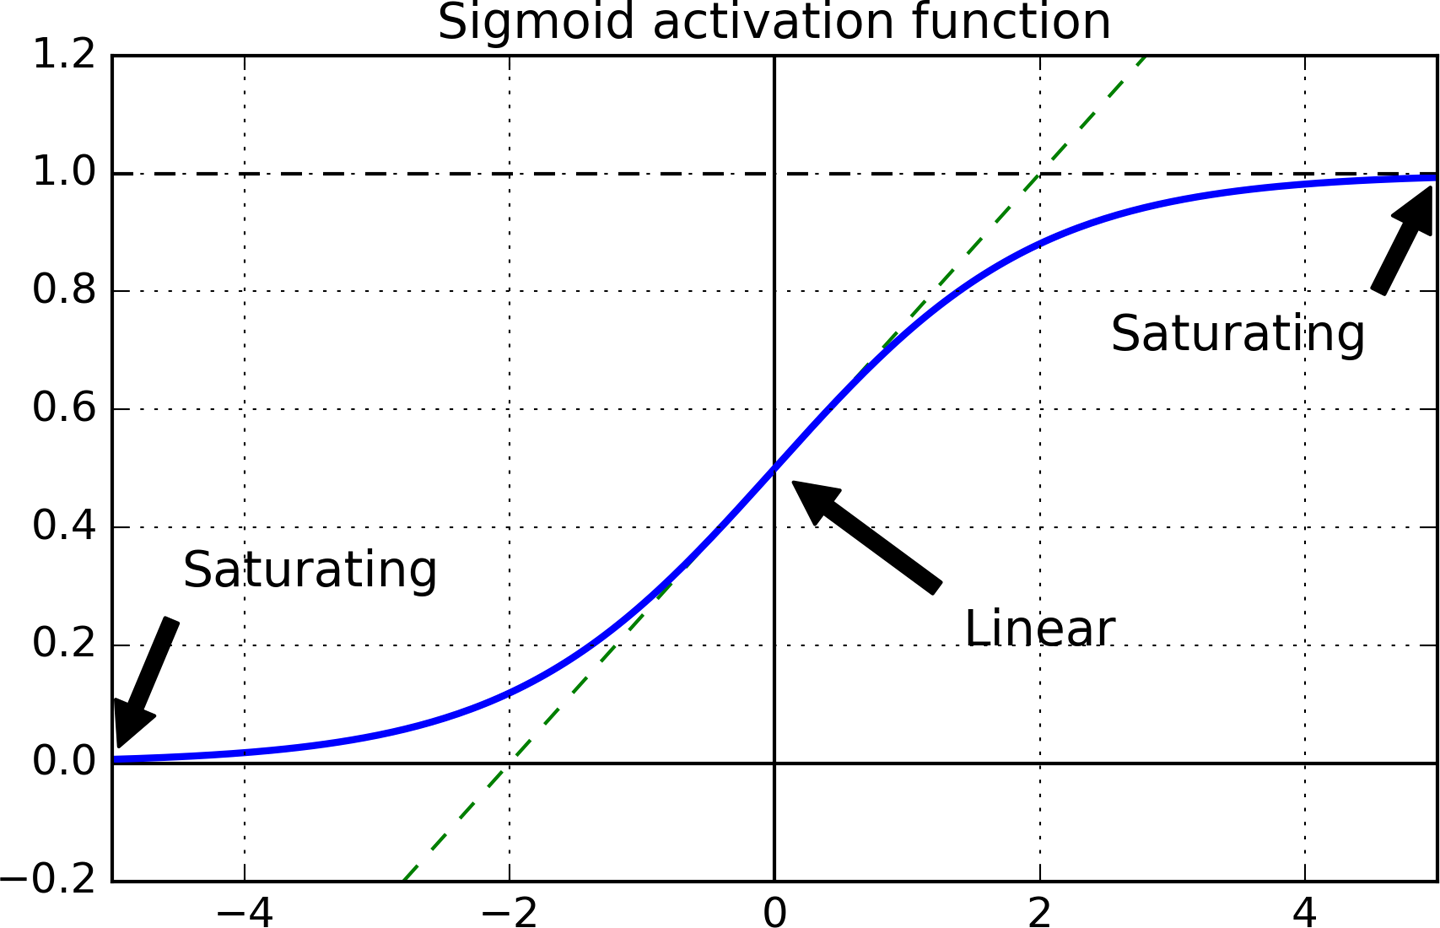
\includegraphics[width=.8\textwidth]{sigmoid_saturation.png}
\end{center}
{\vfill\footnotesize A. Géron, \emph{Hands-On Machine Learning with Scikit-Learn and TensorFlow} 2017}
\end{frame}

\begin{frame}{ReLU}
\alert{Czy ReLU jest odporne na problemy ze znikającym gradientem?}
\[ ReLU(z) = \max\{0, z\} \]
\centering
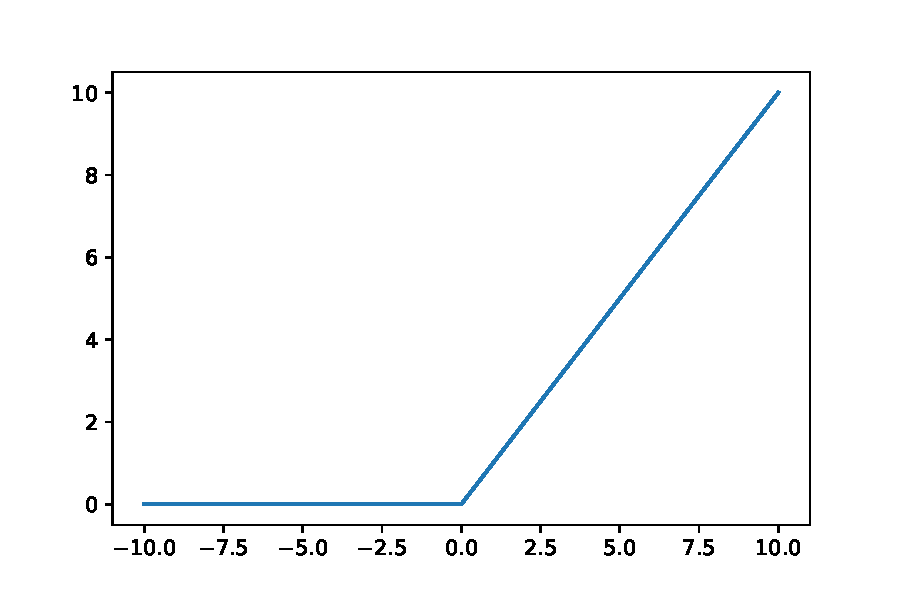
\includegraphics[width=.9\textwidth]{relu.pdf}
\end{frame}

\begin{frame}{Leaky ReLU}
\[ LRelu(z) = \max\{\alpha z, z\} \]
\begin{center}
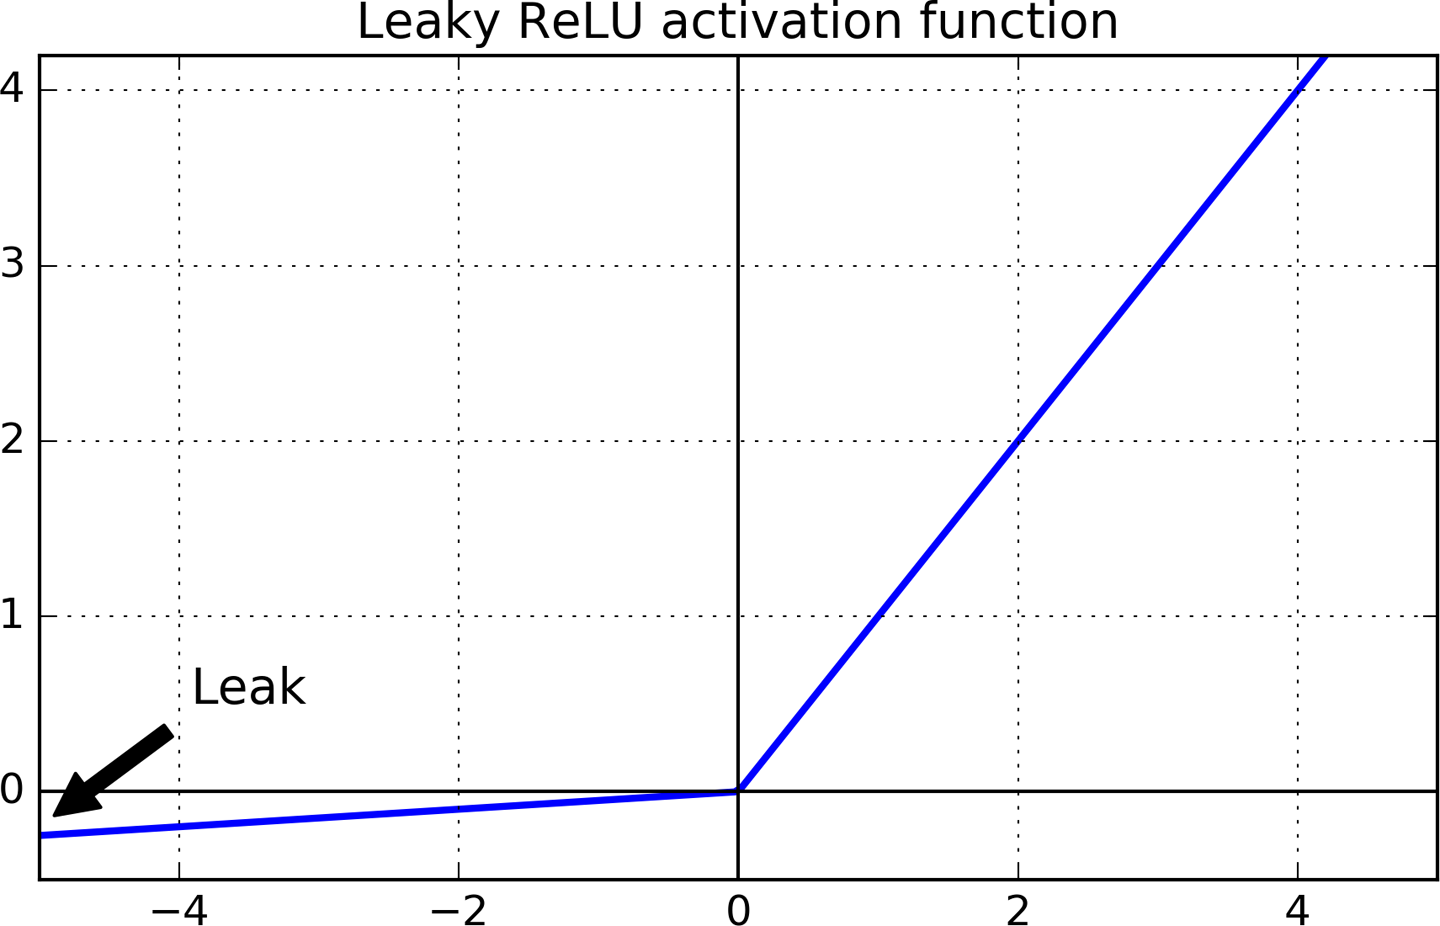
\includegraphics[width=.8\textwidth]{leaky_relu.png}
\end{center}
{\vfill\footnotesize A. Géron, \emph{Hands-On Machine Learning with Scikit-Learn and TensorFlow} 2017}
\note<1>{Typowo $\alpha=0{,}01$, chociaż w niektórych sytuacjach okazuje się, że dużo większa wartość $\alpha=0{,}2$ sprawdza się lepiej}
\end{frame}

\begin{frame}{ELU}
\[ ELU(z) = \begin{cases} \alpha (e^z-1) \qquad z<0 \\ z \qquad z\geq 0 \end{cases} \]
\begin{center}
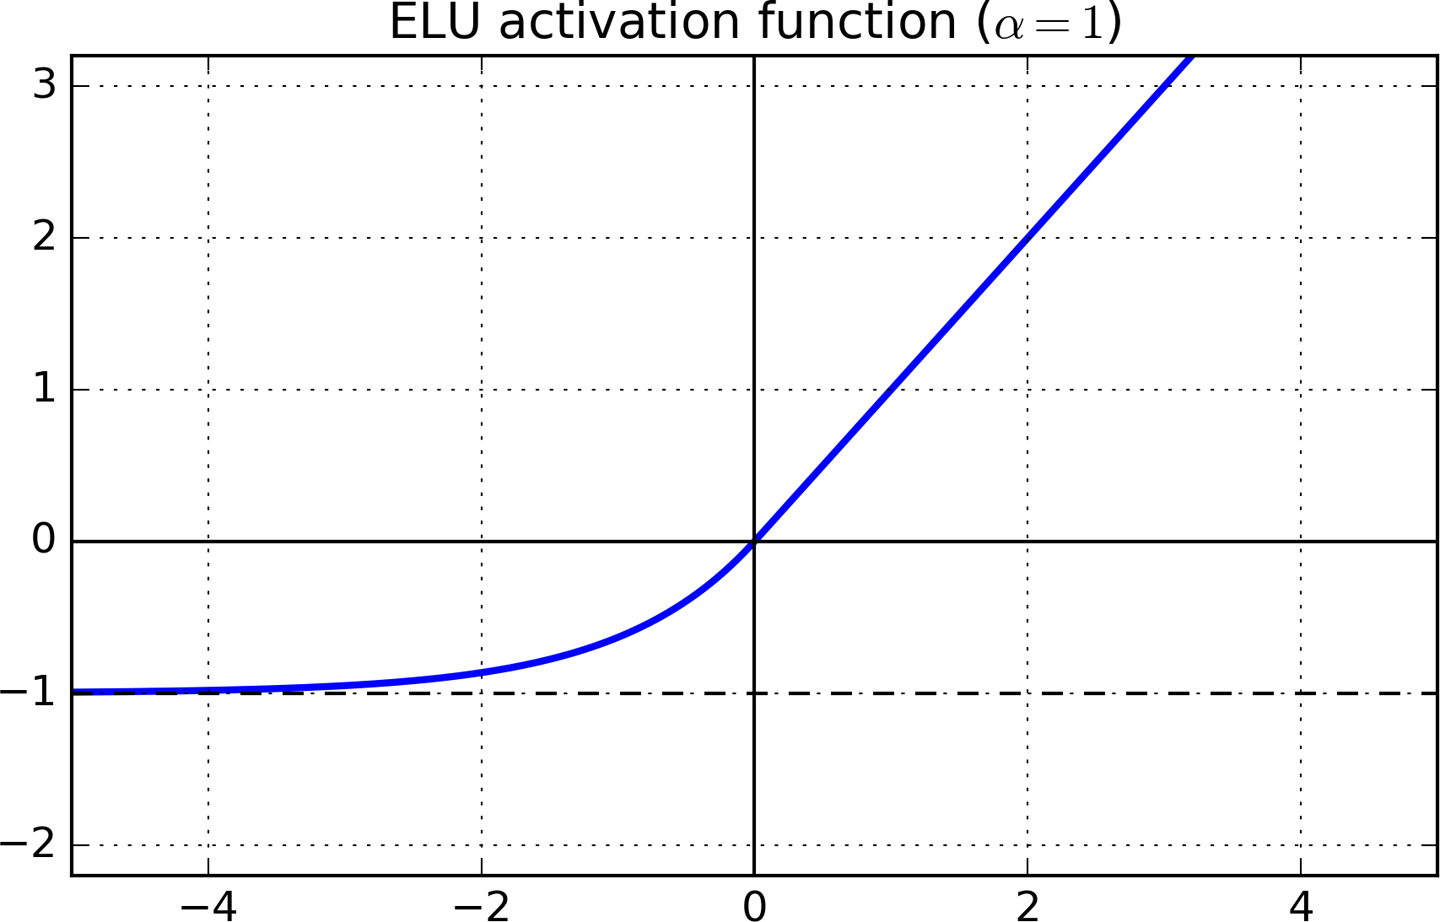
\includegraphics[width=.7\textwidth]{elu.png}
\end{center}
{\vfill\footnotesize A. Géron, \emph{Hands-On Machine Learning with Scikit-Learn and TensorFlow} 2017}
\note<1>{
\begin{itemize}
\item zwykle $\alpha=1$
\item średnia około 0, co pomaga zmniejszyć problem znikającego gradientu
\item gładka, więc w okolicach 0 jest mniej "odbijania" gradientu
\item niezerowy gradient dla $z<0$ 
\end{itemize}
}
\end{frame}

\begin{frame}{Strategia inicjalizacji wag}
\begin{block}{Obserwacja (Xavier Glorot, Yoshua Bengio 2010)}
Wariancja wejść warstwy powinna  być z grubsza równa wariancji wyjść warstwy, a wariancja gradientów przed warstwą wariancji gradientów za warstwą.
\end{block}
\pause
\vfill
\alert{Xavier initialization} \\
\begin{tabular}{p{.27\textwidth}p{.27\textwidth}p{.27\textwidth}}
funkcja aktywacji & rozkład jednostajny $[-r,r]$ & rozkład normalny $N(0, \sigma)$ \\
\hline
logistyczna & $r=\sqrt{\frac{6}{n_{in}+n_{out}}}$ & $\sigma=\sqrt{\frac{2}{n_{in}+n_{out}}}$ \\
tanh & $r=4\sqrt{\frac{6}{n_{in}+n_{out}}}$ & $\sigma=4\sqrt{\frac{2}{n_{in}+n_{out}}}$ \\
ReLU/LReLU/ELU & $r=\sqrt{2}\sqrt{\frac{6}{n_{in}+n_{out}}}$ & $\sigma=\sqrt{2}\sqrt{\frac{2}{n_{in}+n_{out}}}$ \\
\end{tabular}
\end{frame}

\begin{frame}{Batch normalization (Ioffe Szegedy 2015)}
\[\vec{Z} = \vec{Xw} \]
\pause
\[\vec{m_B} = \frac{1}{n} \sum_{i=1}^{n} \vec{Z_i} \]
\pause
\[\vec{s_B}^2 = \frac{1}{n} \sum_{i=1}^{n} \left(\vec{Z_i}-\vec{m_B}\right)^2 \]
\pause
\[\widehat{\vec{Z_i}} = \frac{\vec{Z_i}-\vec{m_B}}{\sqrt{\vec{s_B}^2+\varepsilon}} \]
\pause
\[\vec{\widetilde{Z_i}} = \vec{\gamma} \cdot \widehat{\vec{Z_i}}+\vec{\beta}\]
\pause
\[\vec{Y_i} = f(\vec{\widetilde{Z_i}}) \]
\note<1>
{
W trakcie uczenia $\vec{m_B}$ i $\vec{s_B}$ są obliczane dla każdego minibatch osobno. W trakcie testowania $\vec{m_B}$ i $\vec{s_B}$ to wartości obliczone na całym zbiorze uczącym.
Wektory $\gamma$ i $\beta$ są uczone.

$\cdot$ to iloczyn element po elemencie, a nie wektorowy; $f$ to funkcja aktywacji w danej warstwie, np. ELU
}
\end{frame}

\begin{frame}{Reużywanie NN}
\begin{center}
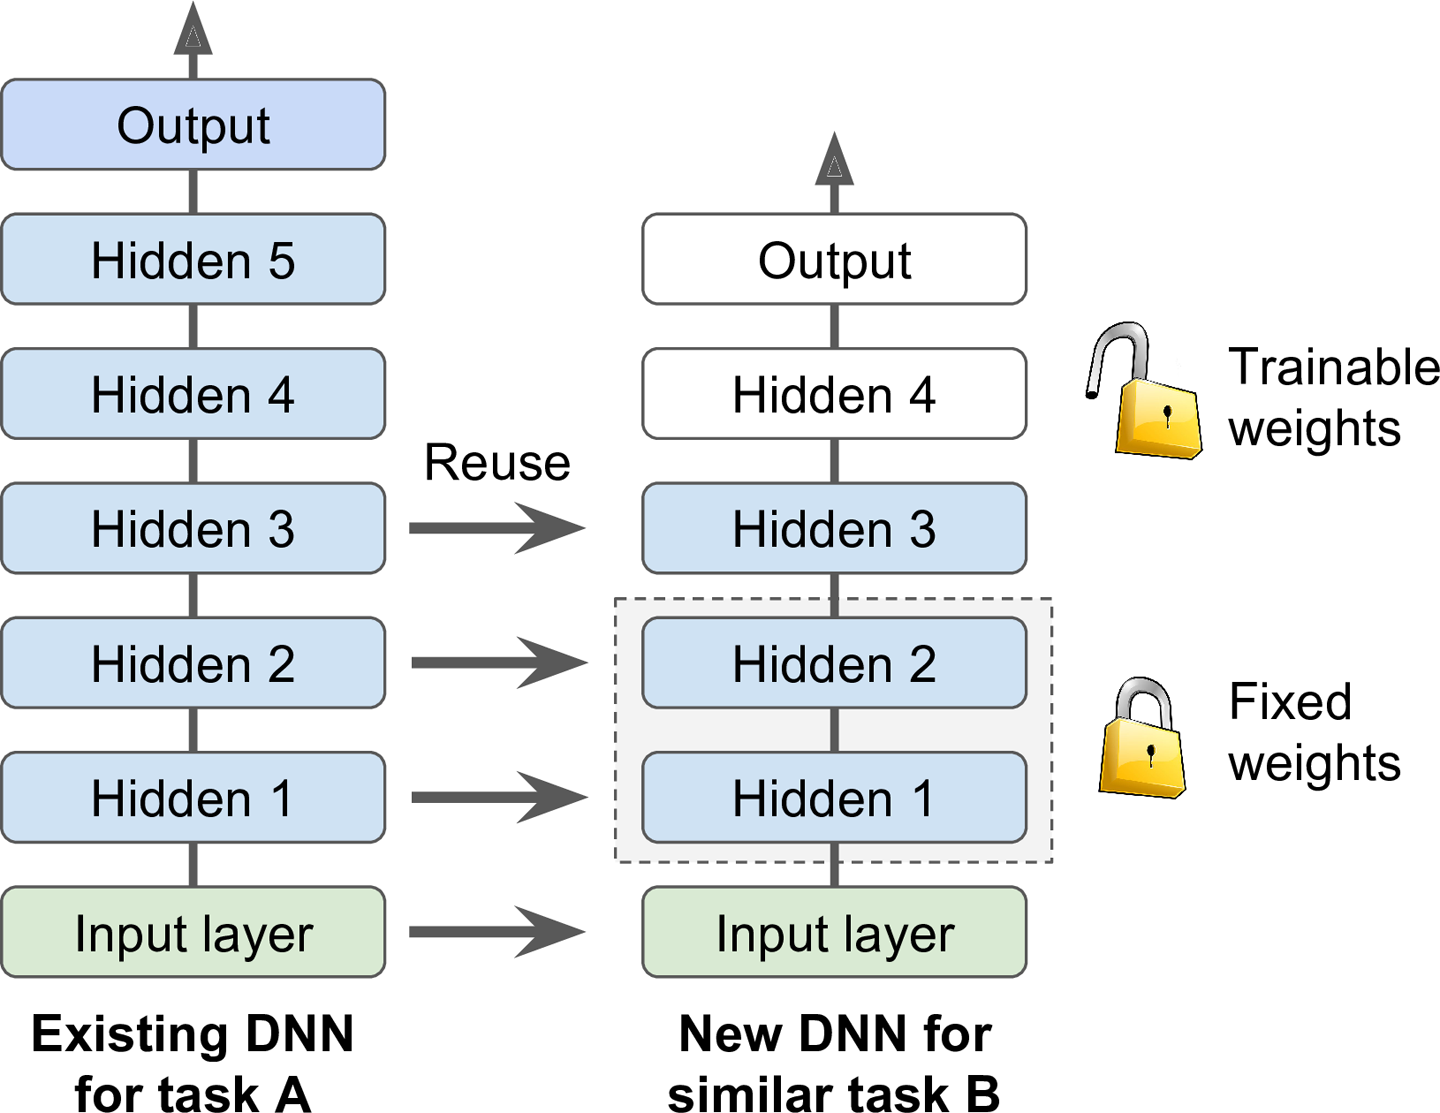
\includegraphics[width=.7\textwidth]{reusing.png}
\end{center}
{\vfill\footnotesize A. Géron, \emph{Hands-On Machine Learning with Scikit-Learn and TensorFlow} 2017}
\end{frame}

\begin{frame}{Regularyzacja}
\begin{itemize}
\item<+-> early stopping
\item<+-> regularyzacja $L_1$ i $L_2$
\item<+-> dropout
\only<.>
{
\\\centering
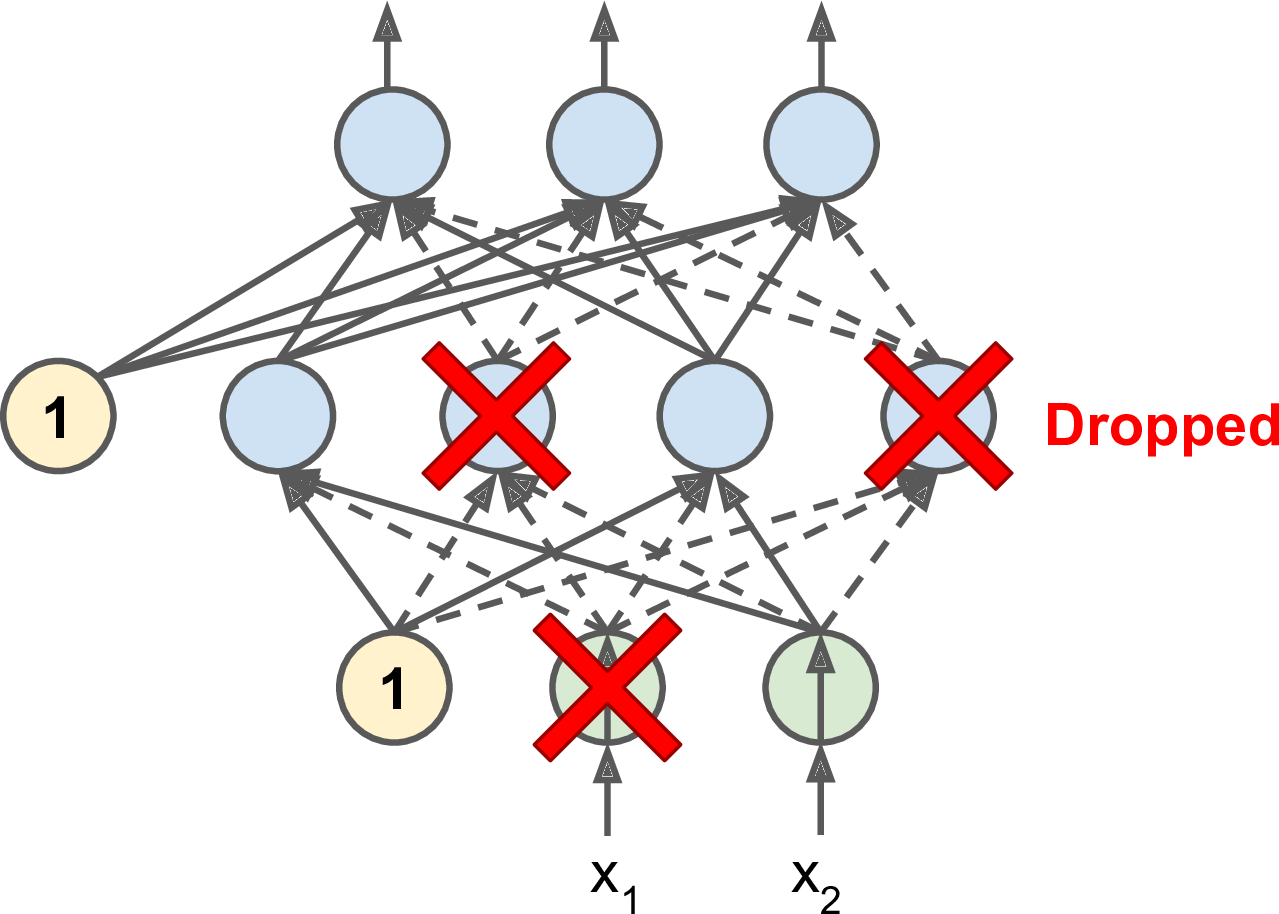
\includegraphics[width=.7\textwidth]{mlst_1109.png}
}
\item<+-> max-norm
\[ \vec{w} = \begin{cases} \vec{w}\frac{r}{\left\|\vec{w}\right\|_2} & \left\|\vec{w}\right\| > r \\ \vec{w} & \left\|\vec{w}\right\| \leq r \end{cases} \]
\end{itemize}
\end{frame}

\end{document}
